\section{Introduction}
Large-scale Transformer-based~\cite{transformer} pre-trained language models~(PLMs)~\cite{bert,roberta,t5}  
have demonstrated state-of-the-art performance across a wide variety of natural language 
processing tasks, including natural language understanding and natural language generation. 
These models are largely over-parametrized~\cite{overpara} in that they usually contain 
hundreds of millions of parameters, rendering them computationally intensive and inefficient in terms 
of both memory and inference latency. Due to this disadvantage, the application of 
PLMs in low-resource scenarios has been restricted.

\begin{figure}[th]
	\centering
	\scalebox{0.115}{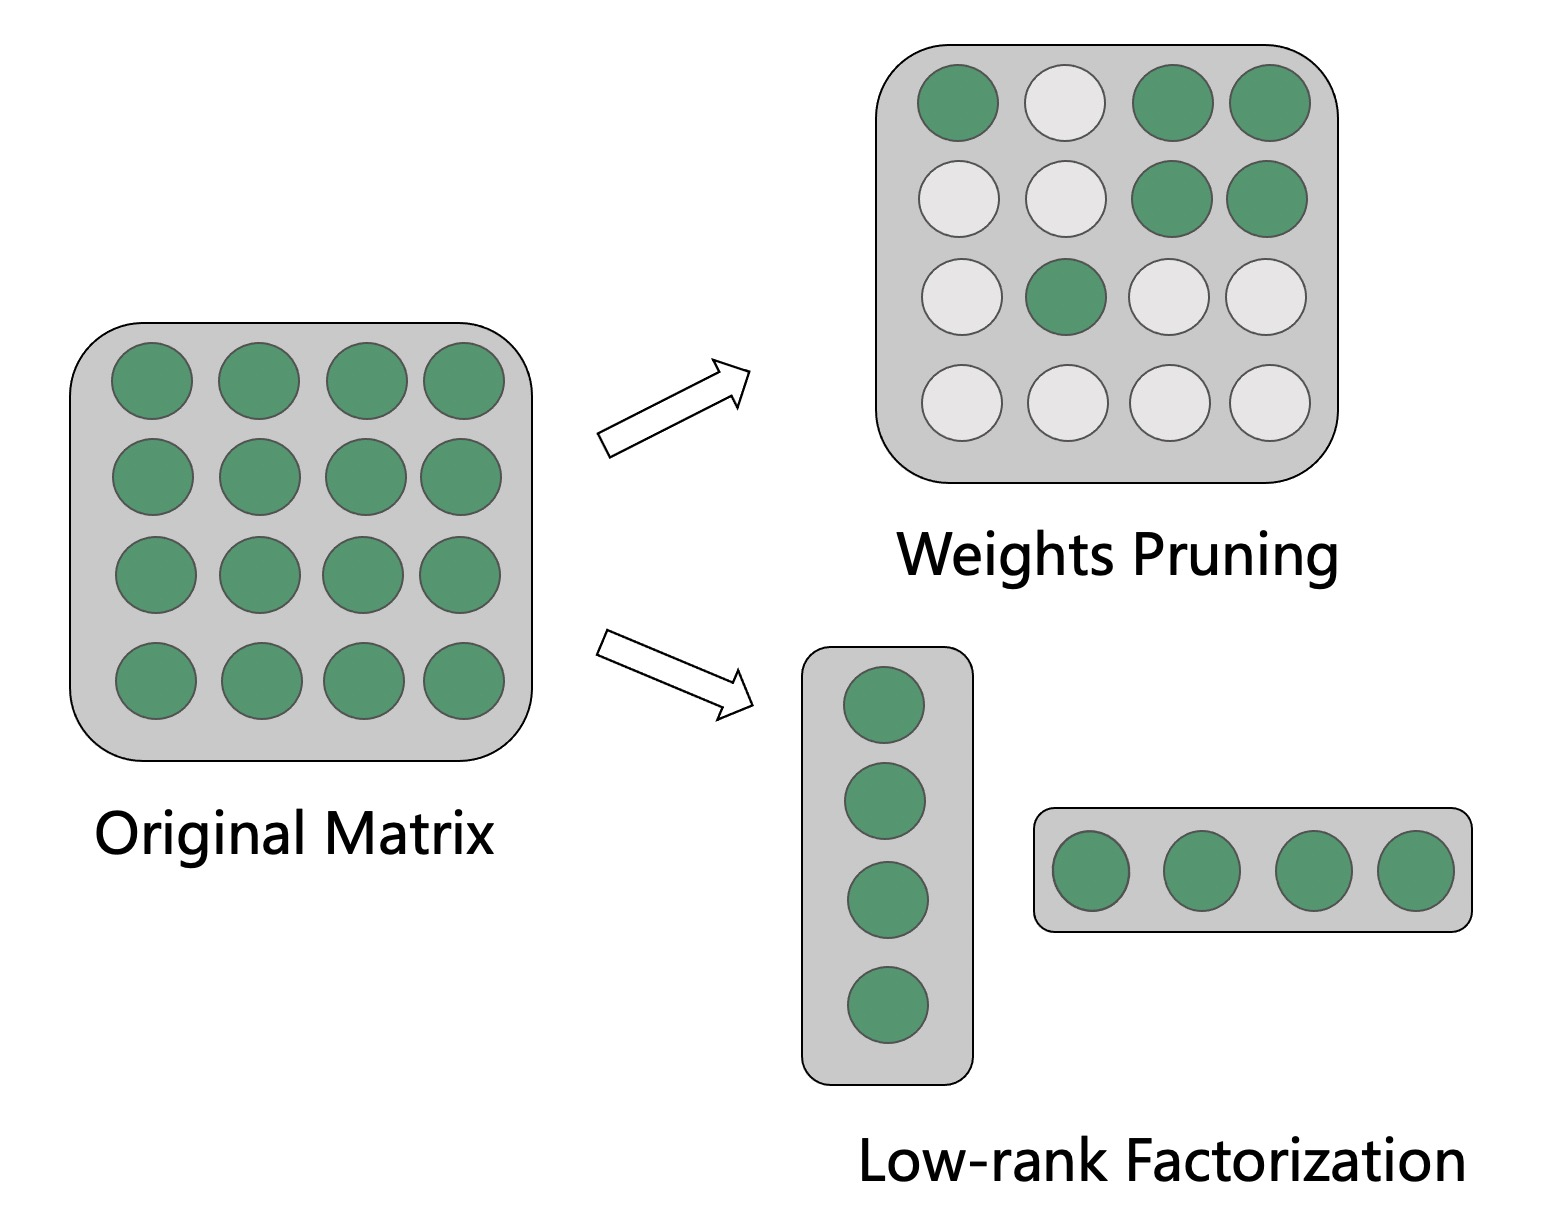
\includegraphics{./figures/intro_3.png}}
	\caption{Illustration of weights pruning and low-rank factorization applied on a single weight matrix.}
	\label{fig:intro}
\end{figure}

To alleviate this problem, model compression~\cite{kd,mag,l0,svd} has emerged as a 
timely research field in recent years. Among all compression techniques, \textit{weights pruning} 
and \textit{low-rank factorization} have received much attention because of their interesting properties.
In weights pruning, model weights are systematically removed by certain pruning criteria, e.g., learnable importance score. Though effective, the resultant unstructured sparse matrices require special linear algebra implementation~\cite{yao} or hardware~\cite{cao} to obtain a perceivable reduction in memory and computation. In contrast, low-rank factorization decomposes the original weight matrix into smaller sub-matrices, providing direct improvement in efficiency. However, it tends to give worse performance than weights pruning given the same parameter budget.

In this work, we first conduct a preliminary study on common weights pruning and low-rank 
factorization methods for better understanding of their mechanisms. 
For weights pruning, we select algorithms with and without using gradient-level information when computing the importance score, denoted as \textit{first-order} and \textit{zero-order} weights pruning. For low-rank factorization, we select singular value decomposition~(SVD) due to its widespread use. From our experiments, we make the following observations: (1) under a high compression ratio, low-rank factorization fails to retain satisfactory performance because the weight matrices of densely fine-tuned models are nearly \textit{full-rank}~(767 on average for BERT-base) and much task-specific information is lost after low-rank approximation; (2) only first-order weights pruning algorithms produces sparse weight matrices that are \textit{low-rank}, showing that gradient information is essential for an accurate indicator of weights importance so as to discover the intrinsic low-rank structure.

The above two findings motivate us to explore the possibility of performing low-rank factorization on low-rank sparse models for effective compression of PLMs. Concretely, for a given PLM and training data, we first apply first-order weights pruning~\cite{movement} on it to obtain its low-rank sparse counterpart. Then, each sparse weight matrix is factorized into two smaller sub-matrices via SVD, which are further fine-tuned to recover full performance. The procedure is 
model architecture-agnostic and hence can be potentially applied to a broad set of existing PLMs. 
%\KZ{While the approach is archi-agnostic and can be applied to different PLMs, it's effectiveness
%is not verified except on BERT-base. I think this is perhaps the only weakness now. Can we do
%some experiments that also works for the two tasks, such as RoBERTa, or XLNet?}
%\KZ{Be careful when you use the word ``architecture'', as you
%mentioned low level matrix computation and hardware before. So does this
%archi mean hardware/systems kind of archi or language model archi?}

Moreover, we noted that the vanilla SVD is not designed for 
sparse matrices because it penalizes the approximation error of 
each parameter equally~\cite{group}. Also, due to the reduced capacity, 
the joint fine-tuning of low-rank sub-matrices may converge to 
solutions with lower generalization performance. To address the first problem, 
we propose sparsity-aware SVD, a weighted variant of SVD that 
better reconstructs unpruned~(hence more important) parameters. 
To address the second problem, we introduce mixed-rank fine-tuning, 
a regularized training scheme where the low-rank sub-matrices 
are randomly replaced with sparse matrix from which they are factorized. 
%\KZ{What 
%do u mean by ``corresponding'' sparse matrix?}


We test on natural language understanding and question answering tasks. Experimental results show that the proposed \textbf{L}ow-rank  \textbf{P}rune-\textbf{A}nd-\textbf{F}actorize~(LPAF) approach can combine the best of both worlds and outperforms existing approaches in terms of compression-performance trade-off. When augmented with sparsity-aware SVD and mixed-rank fine-tuning, the performance is consistently improved. We also conduct in-depth analysis and ablation studies to provide guidance regarding different resource budgets.

Our contributions are summarized as follows:
\begin{itemize}
	\item Through a comprehensive preliminary study, we discover a high-rank phenomenon in models 
produced by fine-tuning/zero-order pruning and a low-rank phenomenon by first-order pruning, 
which highlights the possibility of a more efficient parametrization of low-rank sparse 
matrices using low-rank factorization.
	\item We propose sparsity-aware SVD and mixed-rank fine-tuning to further improve compression performance by prioritizing reconstruction of unpruned weights at initialization and compensating for the reduced capacity during training respectively.
	\item Experiments on natural language understanding and question answering tasks show that our method can achieve a 5.4x-12.3x reduction in model size and 4.6x-10.6x reduction in computation cost while retaining 98\%-93\% of the performance of the original BERT.
\end{itemize}
